\documentclass[]{article}
\usepackage{lmodern}
\usepackage{amssymb,amsmath}
\usepackage{ifxetex,ifluatex}
\usepackage{fixltx2e} % provides \textsubscript
\ifnum 0\ifxetex 1\fi\ifluatex 1\fi=0 % if pdftex
  \usepackage[T1]{fontenc}
  \usepackage[utf8]{inputenc}
\else % if luatex or xelatex
  \ifxetex
    \usepackage{mathspec}
  \else
    \usepackage{fontspec}
  \fi
  \defaultfontfeatures{Ligatures=TeX,Scale=MatchLowercase}
\fi
% use upquote if available, for straight quotes in verbatim environments
\IfFileExists{upquote.sty}{\usepackage{upquote}}{}
% use microtype if available
\IfFileExists{microtype.sty}{%
\usepackage{microtype}
\UseMicrotypeSet[protrusion]{basicmath} % disable protrusion for tt fonts
}{}
\usepackage[margin=1in]{geometry}
\usepackage{hyperref}
\hypersetup{unicode=true,
            pdftitle={Conservancy Analysis},
            pdfauthor={BEACN},
            pdfborder={0 0 0},
            breaklinks=true}
\urlstyle{same}  % don't use monospace font for urls
\usepackage{color}
\usepackage{fancyvrb}
\newcommand{\VerbBar}{|}
\newcommand{\VERB}{\Verb[commandchars=\\\{\}]}
\DefineVerbatimEnvironment{Highlighting}{Verbatim}{commandchars=\\\{\}}
% Add ',fontsize=\small' for more characters per line
\usepackage{framed}
\definecolor{shadecolor}{RGB}{248,248,248}
\newenvironment{Shaded}{\begin{snugshade}}{\end{snugshade}}
\newcommand{\KeywordTok}[1]{\textcolor[rgb]{0.13,0.29,0.53}{\textbf{#1}}}
\newcommand{\DataTypeTok}[1]{\textcolor[rgb]{0.13,0.29,0.53}{#1}}
\newcommand{\DecValTok}[1]{\textcolor[rgb]{0.00,0.00,0.81}{#1}}
\newcommand{\BaseNTok}[1]{\textcolor[rgb]{0.00,0.00,0.81}{#1}}
\newcommand{\FloatTok}[1]{\textcolor[rgb]{0.00,0.00,0.81}{#1}}
\newcommand{\ConstantTok}[1]{\textcolor[rgb]{0.00,0.00,0.00}{#1}}
\newcommand{\CharTok}[1]{\textcolor[rgb]{0.31,0.60,0.02}{#1}}
\newcommand{\SpecialCharTok}[1]{\textcolor[rgb]{0.00,0.00,0.00}{#1}}
\newcommand{\StringTok}[1]{\textcolor[rgb]{0.31,0.60,0.02}{#1}}
\newcommand{\VerbatimStringTok}[1]{\textcolor[rgb]{0.31,0.60,0.02}{#1}}
\newcommand{\SpecialStringTok}[1]{\textcolor[rgb]{0.31,0.60,0.02}{#1}}
\newcommand{\ImportTok}[1]{#1}
\newcommand{\CommentTok}[1]{\textcolor[rgb]{0.56,0.35,0.01}{\textit{#1}}}
\newcommand{\DocumentationTok}[1]{\textcolor[rgb]{0.56,0.35,0.01}{\textbf{\textit{#1}}}}
\newcommand{\AnnotationTok}[1]{\textcolor[rgb]{0.56,0.35,0.01}{\textbf{\textit{#1}}}}
\newcommand{\CommentVarTok}[1]{\textcolor[rgb]{0.56,0.35,0.01}{\textbf{\textit{#1}}}}
\newcommand{\OtherTok}[1]{\textcolor[rgb]{0.56,0.35,0.01}{#1}}
\newcommand{\FunctionTok}[1]{\textcolor[rgb]{0.00,0.00,0.00}{#1}}
\newcommand{\VariableTok}[1]{\textcolor[rgb]{0.00,0.00,0.00}{#1}}
\newcommand{\ControlFlowTok}[1]{\textcolor[rgb]{0.13,0.29,0.53}{\textbf{#1}}}
\newcommand{\OperatorTok}[1]{\textcolor[rgb]{0.81,0.36,0.00}{\textbf{#1}}}
\newcommand{\BuiltInTok}[1]{#1}
\newcommand{\ExtensionTok}[1]{#1}
\newcommand{\PreprocessorTok}[1]{\textcolor[rgb]{0.56,0.35,0.01}{\textit{#1}}}
\newcommand{\AttributeTok}[1]{\textcolor[rgb]{0.77,0.63,0.00}{#1}}
\newcommand{\RegionMarkerTok}[1]{#1}
\newcommand{\InformationTok}[1]{\textcolor[rgb]{0.56,0.35,0.01}{\textbf{\textit{#1}}}}
\newcommand{\WarningTok}[1]{\textcolor[rgb]{0.56,0.35,0.01}{\textbf{\textit{#1}}}}
\newcommand{\AlertTok}[1]{\textcolor[rgb]{0.94,0.16,0.16}{#1}}
\newcommand{\ErrorTok}[1]{\textcolor[rgb]{0.64,0.00,0.00}{\textbf{#1}}}
\newcommand{\NormalTok}[1]{#1}
\usepackage{graphicx,grffile}
\makeatletter
\def\maxwidth{\ifdim\Gin@nat@width>\linewidth\linewidth\else\Gin@nat@width\fi}
\def\maxheight{\ifdim\Gin@nat@height>\textheight\textheight\else\Gin@nat@height\fi}
\makeatother
% Scale images if necessary, so that they will not overflow the page
% margins by default, and it is still possible to overwrite the defaults
% using explicit options in \includegraphics[width, height, ...]{}
\setkeys{Gin}{width=\maxwidth,height=\maxheight,keepaspectratio}
\IfFileExists{parskip.sty}{%
\usepackage{parskip}
}{% else
\setlength{\parindent}{0pt}
\setlength{\parskip}{6pt plus 2pt minus 1pt}
}
\setlength{\emergencystretch}{3em}  % prevent overfull lines
\providecommand{\tightlist}{%
  \setlength{\itemsep}{0pt}\setlength{\parskip}{0pt}}
\setcounter{secnumdepth}{0}
% Redefines (sub)paragraphs to behave more like sections
\ifx\paragraph\undefined\else
\let\oldparagraph\paragraph
\renewcommand{\paragraph}[1]{\oldparagraph{#1}\mbox{}}
\fi
\ifx\subparagraph\undefined\else
\let\oldsubparagraph\subparagraph
\renewcommand{\subparagraph}[1]{\oldsubparagraph{#1}\mbox{}}
\fi

%%% Use protect on footnotes to avoid problems with footnotes in titles
\let\rmarkdownfootnote\footnote%
\def\footnote{\protect\rmarkdownfootnote}

%%% Change title format to be more compact
\usepackage{titling}

% Create subtitle command for use in maketitle
\newcommand{\subtitle}[1]{
  \posttitle{
    \begin{center}\large#1\end{center}
    }
}

\setlength{\droptitle}{-2em}
  \title{Conservancy Analysis}
  \pretitle{\vspace{\droptitle}\centering\huge}
  \posttitle{\par}
  \author{BEACN}
  \preauthor{\centering\large\emph}
  \postauthor{\par}
  \predate{\centering\large\emph}
  \postdate{\par}
  \date{March 23, 2018}


\begin{document}
\maketitle

\subsection{Setup}\label{setup}

Downloading the data

\begin{Shaded}
\begin{Highlighting}[]
\KeywordTok{library}\NormalTok{(tidyverse)}
\end{Highlighting}
\end{Shaded}

\begin{verbatim}
## -- Attaching packages ----------------------------------------------------------------------------------------- tidyverse 1.2.1 --
\end{verbatim}

\begin{verbatim}
## v ggplot2 2.2.1.9000     v purrr   0.2.4     
## v tibble  1.4.2          v dplyr   0.7.4     
## v tidyr   0.7.2          v stringr 1.2.0     
## v readr   1.1.1          v forcats 0.2.0
\end{verbatim}

\begin{verbatim}
## -- Conflicts -------------------------------------------------------------------------------------------- tidyverse_conflicts() --
## x dplyr::filter() masks stats::filter()
## x dplyr::lag()    masks stats::lag()
## x dplyr::vars()   masks ggplot2::vars()
\end{verbatim}

\begin{Shaded}
\begin{Highlighting}[]
\KeywordTok{library}\NormalTok{(ggplot2)}
\KeywordTok{library}\NormalTok{(stringr)}
\KeywordTok{library}\NormalTok{(gridExtra)}
\end{Highlighting}
\end{Shaded}

\begin{verbatim}
## Warning: package 'gridExtra' was built under R version 3.4.4
\end{verbatim}

\begin{verbatim}
## 
## Attaching package: 'gridExtra'
\end{verbatim}

\begin{verbatim}
## The following object is masked from 'package:dplyr':
## 
##     combine
\end{verbatim}

\begin{Shaded}
\begin{Highlighting}[]
\KeywordTok{library}\NormalTok{(grid)}

\NormalTok{conservancy_names <-}\StringTok{ }\ControlFlowTok{function}\NormalTok{(name) \{}
  \KeywordTok{return}\NormalTok{(}\KeywordTok{paste0}\NormalTok{(}\StringTok{"conservancy_"}\NormalTok{, name, }\StringTok{".csv"}\NormalTok{)) }
\NormalTok{\}}

\NormalTok{ucnrs_names <-}\StringTok{ }\ControlFlowTok{function}\NormalTok{(name) \{}
  \KeywordTok{return}\NormalTok{(}\KeywordTok{paste0}\NormalTok{(}\StringTok{"ucnrs_"}\NormalTok{, name, }\StringTok{".csv"}\NormalTok{))}
\NormalTok{\}}

\NormalTok{conservancyNames <-}\StringTok{ }\KeywordTok{c}\NormalTok{(}\StringTok{"birds"}\NormalTok{, }\StringTok{"herpetofauna"}\NormalTok{, }\StringTok{"invertebrates"}\NormalTok{, }\StringTok{"mammals"}\NormalTok{, }\StringTok{"plants"}\NormalTok{)}

\NormalTok{ucnrsNames <-}\StringTok{ }\KeywordTok{c}\NormalTok{(}\StringTok{"animal_list"}\NormalTok{, }\StringTok{"plant_list"}\NormalTok{)}

\NormalTok{fullConservancyNames <-}\StringTok{ }\KeywordTok{conservancy_names}\NormalTok{(conservancyNames)}
\NormalTok{fullUCNRSNames <-}\StringTok{ }\KeywordTok{ucnrs_names}\NormalTok{(ucnrsNames)}

\NormalTok{allFiles <-}\StringTok{ }\KeywordTok{c}\NormalTok{(fullConservancyNames, fullUCNRSNames)}
\NormalTok{path <-}\StringTok{ }\KeywordTok{paste0}\NormalTok{(}\StringTok{"./ucnrs_data/"}\NormalTok{, allFiles)}

\NormalTok{data <-}\StringTok{ }\KeywordTok{lapply}\NormalTok{(path, read_csv) }
\end{Highlighting}
\end{Shaded}

\begin{verbatim}
## Parsed with column specification:
## cols(
##   species = col_character()
## )
\end{verbatim}

\begin{verbatim}
## Parsed with column specification:
## cols(
##   species = col_character()
## )
\end{verbatim}

\begin{verbatim}
## Parsed with column specification:
## cols(
##   Species = col_character()
## )
\end{verbatim}

\begin{verbatim}
## Parsed with column specification:
## cols(
##   species = col_character()
## )
## Parsed with column specification:
## cols(
##   species = col_character()
## )
\end{verbatim}

\begin{verbatim}
## Parsed with column specification:
## cols(
##   Reserve = col_character(),
##   Taxon = col_character(),
##   Family = col_character(),
##   `Scientific Name` = col_character(),
##   `Accepted Name` = col_character(),
##   `Common Name` = col_character()
## )
\end{verbatim}

\begin{verbatim}
## Warning: Missing column names filled in: 'X17' [17], 'X18' [18],
## 'X19' [19], 'X20' [20], 'X21' [21], 'X22' [22]
\end{verbatim}

\begin{verbatim}
## Parsed with column specification:
## cols(
##   .default = col_character(),
##   `Reserve count (values)` = col_integer(),
##   `Reserve count (formula)` = col_integer()
## )
\end{verbatim}

\begin{verbatim}
## See spec(...) for full column specifications.
\end{verbatim}

\begin{Shaded}
\begin{Highlighting}[]
\KeywordTok{head}\NormalTok{(data)}
\end{Highlighting}
\end{Shaded}

\subsection{Combining UCNRS and Conservancy into four
datasets}\label{combining-ucnrs-and-conservancy-into-four-datasets}

\begin{Shaded}
\begin{Highlighting}[]
\CommentTok{# Separating out columns of data for conservancy data and removing irrelevant values}

\NormalTok{conservancyAnimalData <-}\StringTok{ }\KeywordTok{bind_rows}\NormalTok{(data[[}\DecValTok{1}\NormalTok{]], data[[}\DecValTok{2}\NormalTok{]], data[[}\DecValTok{3}\NormalTok{]], data[[}\DecValTok{4}\NormalTok{]]) }\OperatorTok\StringTok{ }
\StringTok{  }\KeywordTok{distinct}\NormalTok{(species) }\OperatorTok\StringTok{ }
\StringTok{  }\KeywordTok{separate}\NormalTok{(species, }\DataTypeTok{into =} \KeywordTok{c}\NormalTok{(}\StringTok{"genus"}\NormalTok{, }\StringTok{"species"}\NormalTok{, }\StringTok{"sublabel1"}\NormalTok{, }\StringTok{"sublabel2"}\NormalTok{), }\DataTypeTok{sep =} \StringTok{" "}\NormalTok{, }\DataTypeTok{extra =} \StringTok{"merge"}\NormalTok{) }\OperatorTok\StringTok{ }
\StringTok{  }\KeywordTok{filter}\NormalTok{(}\OperatorTok{!}\NormalTok{(genus }\OperatorTok\StringTok{ }\KeywordTok{c}\NormalTok{(}\StringTok{"Tejon"}\NormalTok{, }\StringTok{"Undefined"}\NormalTok{)))}
\end{Highlighting}
\end{Shaded}

\begin{verbatim}
## Warning: Too few values at 351 locations: 1, 2, 3, 4, 5, 6, 7, 8, 9, 10,
## 11, 12, 13, 14, 15, 16, 17, 18, 19, 20, ...
\end{verbatim}

\begin{Shaded}
\begin{Highlighting}[]
\NormalTok{conservancyPlantData <-}\StringTok{ }\NormalTok{data[[}\DecValTok{5}\NormalTok{]] }\OperatorTok\StringTok{ }\KeywordTok{distinct}\NormalTok{(species) }\OperatorTok\StringTok{ }
\StringTok{  }\KeywordTok{separate}\NormalTok{(species, }\DataTypeTok{into =} \KeywordTok{c}\NormalTok{(}\StringTok{"genus"}\NormalTok{, }\StringTok{"species"}\NormalTok{, }\StringTok{"separator_label"}\NormalTok{, }\StringTok{"sublabel"}\NormalTok{), }\DataTypeTok{sep =} \StringTok{" "}\NormalTok{, }\DataTypeTok{extra =} \StringTok{"merge"}\NormalTok{) }\OperatorTok\StringTok{ }
\StringTok{  }\KeywordTok{filter}\NormalTok{(}\OperatorTok{!}\NormalTok{(genus }\OperatorTok\StringTok{ }\KeywordTok{c}\NormalTok{(}\StringTok{"Tejon"}\NormalTok{, }\StringTok{"Undefined"}\NormalTok{)))}
\end{Highlighting}
\end{Shaded}

\begin{verbatim}
## Warning: Too few values at 652 locations: 2, 4, 5, 6, 11, 12, 13, 14, 15,
## 16, 17, 18, 19, 20, 21, 22, 23, 24, 25, 26, ...
\end{verbatim}

\begin{Shaded}
\begin{Highlighting}[]
\CommentTok{# Loading Plant and Animal data from UCNRS}

\NormalTok{ucnrsPlantData <-}\StringTok{ }\NormalTok{data[[}\DecValTok{7}\NormalTok{]]}
\NormalTok{ucnrsAnimalData <-}\StringTok{ }\NormalTok{data[[}\DecValTok{6}\NormalTok{]]}

\CommentTok{# Relabeling data}

\KeywordTok{names}\NormalTok{(ucnrsPlantData)[}\DecValTok{7}\OperatorTok{:}\DecValTok{8}\NormalTok{] <-}\StringTok{ }\KeywordTok{c}\NormalTok{(}\StringTok{"separator_label"}\NormalTok{, }\StringTok{"sublabel"}\NormalTok{)}
\KeywordTok{names}\NormalTok{(ucnrsAnimalData)[}\DecValTok{4}\NormalTok{] <-}\StringTok{ "scientific_name"}

\CommentTok{# Cleaning UCNRS Animal data}

\NormalTok{ucnrsAnimalDataSubsetTemp <-}\StringTok{ }\NormalTok{ucnrsAnimalData }\OperatorTok\StringTok{ }
\StringTok{  }\KeywordTok{select}\NormalTok{(Reserve, scientific_name) }\OperatorTok\StringTok{ }
\StringTok{  }\KeywordTok{separate}\NormalTok{(scientific_name, }\DataTypeTok{into =} \KeywordTok{c}\NormalTok{(}\StringTok{"genus"}\NormalTok{, }\StringTok{"species"}\NormalTok{, }\StringTok{"sublabel1"}\NormalTok{, }\StringTok{"sublabel2"}\NormalTok{), }\DataTypeTok{sep =} \StringTok{" "}\NormalTok{, }\DataTypeTok{extra =} \StringTok{"merge"}\NormalTok{) }\OperatorTok
\StringTok{  }\KeywordTok{distinct}\NormalTok{()}
\end{Highlighting}
\end{Shaded}

\begin{verbatim}
## Warning: Too few values at 8696 locations: 1, 2, 3, 4, 5, 6, 7, 8, 9, 10,
## 11, 12, 13, 14, 15, 16, 17, 18, 19, 20, ...
\end{verbatim}

\begin{Shaded}
\begin{Highlighting}[]
\NormalTok{ucnrsAnimalDataSubset <-}\StringTok{  }\KeywordTok{mutate}\NormalTok{(ucnrsAnimalDataSubsetTemp, }
                                 \DataTypeTok{sublabel1 =} \KeywordTok{gsub}\NormalTok{(}\StringTok{"}\CharTok{\textbackslash{}\textbackslash{}}\StringTok{("}\NormalTok{, }\StringTok{""}\NormalTok{, sublabel1), }\DataTypeTok{sublabel2 =} \KeywordTok{gsub}\NormalTok{(}\StringTok{"}\CharTok{\textbackslash{}\textbackslash{}}\StringTok{("}\NormalTok{, }\StringTok{""}\NormalTok{, sublabel2), }
         \DataTypeTok{sublabel1 =} \KeywordTok{gsub}\NormalTok{(}\StringTok{"}\CharTok{\textbackslash{}\textbackslash{}}\StringTok{)"}\NormalTok{, }\StringTok{""}\NormalTok{, sublabel1), }\DataTypeTok{sublabel2 =} \KeywordTok{gsub}\NormalTok{(}\StringTok{"}\CharTok{\textbackslash{}\textbackslash{}}\StringTok{)"}\NormalTok{, }\StringTok{""}\NormalTok{, sublabel2),}
         \DataTypeTok{sublabel1 =} \KeywordTok{gsub}\NormalTok{(}\StringTok{"}\CharTok{\textbackslash{}\textbackslash{}}\StringTok{."}\NormalTok{, }\StringTok{""}\NormalTok{, sublabel1), }\DataTypeTok{sublabel2 =} \KeywordTok{gsub}\NormalTok{(}\StringTok{"}\CharTok{\textbackslash{}\textbackslash{}}\StringTok{."}\NormalTok{, }\StringTok{""}\NormalTok{, sublabel2), }
         \DataTypeTok{species =} \KeywordTok{tolower}\NormalTok{(species))}

\CommentTok{# Cleaning UCNRS Plant Data}

\NormalTok{ucnrsPlantDataSubset <-}\StringTok{ }\NormalTok{ucnrsPlantData }\OperatorTok\StringTok{ }
\StringTok{  }\KeywordTok{select}\NormalTok{(Reserve, Genus, Species, separator_label, sublabel) }\OperatorTok
\StringTok{  }\KeywordTok{distinct}\NormalTok{()}

\CommentTok{# Relabeling column headers}

\KeywordTok{names}\NormalTok{(ucnrsPlantDataSubset)[}\DecValTok{1}\OperatorTok{:}\DecValTok{3}\NormalTok{] <-}\StringTok{ }\KeywordTok{c}\NormalTok{(}\StringTok{"reserve"}\NormalTok{, }\StringTok{"genus"}\NormalTok{, }\StringTok{"species"}\NormalTok{)}
\KeywordTok{names}\NormalTok{(ucnrsAnimalDataSubset)[}\DecValTok{1}\NormalTok{] <-}\StringTok{ }\KeywordTok{c}\NormalTok{(}\StringTok{"reserve"}\NormalTok{)}

\CommentTok{# Print results}

\KeywordTok{head}\NormalTok{(ucnrsAnimalDataSubset)}
\end{Highlighting}
\end{Shaded}

\begin{verbatim}
## # A tibble: 6 x 5
##   reserve                    genus         species     sublabel1 sublabel2
##   <chr>                      <chr>         <chr>       <chr>     <chr>    
## 1 Angelo Coast Range Reserve Ambystoma     gracile     <NA>      <NA>     
## 2 Angelo Coast Range Reserve Aneides       ferreus     <NA>      <NA>     
## 3 Angelo Coast Range Reserve Aneides       flavipunct~ <NA>      <NA>     
## 4 Angelo Coast Range Reserve Aneides       vagrans     <NA>      <NA>     
## 5 Angelo Coast Range Reserve Ascaphus      truei       <NA>      <NA>     
## 6 Angelo Coast Range Reserve Bactrachoseps attenuatus  <NA>      <NA>
\end{verbatim}

\begin{Shaded}
\begin{Highlighting}[]
\KeywordTok{head}\NormalTok{(ucnrsPlantDataSubset)}
\end{Highlighting}
\end{Shaded}

\begin{verbatim}
## # A tibble: 6 x 5
##   reserve                     genus   species   separator_label sublabel 
##   <chr>                       <chr>   <chr>     <chr>           <chr>    
## 1 Landells-Hill Big Creek     Abies   bracteata <NA>            <NA>     
## 2 James San Jacinto Mountains Abies   concolor  <NA>            <NA>     
## 3 Valentine                   Abies   concolor  <NA>            <NA>     
## 4 Valentine                   Abies   magnifica var.            magnifica
## 5 Bodega                      Abronia latifolia <NA>            <NA>     
## 6 Younger Lagoon              Abronia latifolia <NA>            <NA>
\end{verbatim}

\begin{Shaded}
\begin{Highlighting}[]
\KeywordTok{head}\NormalTok{(conservancyAnimalData)}
\end{Highlighting}
\end{Shaded}

\begin{verbatim}
## # A tibble: 6 x 4
##   genus species    sublabel1 sublabel2
##   <chr> <chr>      <chr>     <chr>    
## 1 Aix   sponsa     <NA>      <NA>     
## 2 Anas  acuta      <NA>      <NA>     
## 3 Anas  americana  <NA>      <NA>     
## 4 Anas  clypeata   <NA>      <NA>     
## 5 Anas  crecca     <NA>      <NA>     
## 6 Anas  cyanoptera <NA>      <NA>
\end{verbatim}

\begin{Shaded}
\begin{Highlighting}[]
\KeywordTok{head}\NormalTok{(conservancyPlantData)}
\end{Highlighting}
\end{Shaded}

\begin{verbatim}
## # A tibble: 6 x 4
##   genus        species      separator_label sublabel    
##   <chr>        <chr>        <chr>           <chr>       
## 1 Sambucus     nigra        subsp.          caerulea    
## 2 Apocynum     cannabinum   <NA>            <NA>        
## 3 Chlorogalum  pomeridianum var.            pomeridianum
## 4 Hesperoyucca whipplei     <NA>            <NA>        
## 5 Yucca        brevifolia   <NA>            <NA>        
## 6 Allium       burlewii     <NA>            <NA>
\end{verbatim}

\subsection{Match Ratio of Plants per
Reserve}\label{match-ratio-of-plants-per-reserve}

\begin{Shaded}
\begin{Highlighting}[]
\CommentTok{# Find shared genies and species of plants}
\NormalTok{matchingPlants <-}\StringTok{ }\KeywordTok{semi_join}\NormalTok{(ucnrsPlantDataSubset, conservancyPlantData, }\DataTypeTok{by =} \KeywordTok{c}\NormalTok{(}\StringTok{"genus"}\NormalTok{, }\StringTok{"species"}\NormalTok{, }\StringTok{"sublabel"}\NormalTok{)) }\OperatorTok
\StringTok{  }\KeywordTok{select}\NormalTok{(reserve, genus, species, sublabel)}

\CommentTok{# Calculate how similar plant species composition is by reserve}
\NormalTok{matchingPlantsCount <-}\StringTok{ }\NormalTok{matchingPlants }\OperatorTok\StringTok{ }
\StringTok{  }\KeywordTok{group_by}\NormalTok{(reserve) }\OperatorTok\StringTok{ }
\StringTok{  }\KeywordTok{summarize}\NormalTok{(}\DataTypeTok{count =} \KeywordTok{n}\NormalTok{())}

\NormalTok{totalPlantsCount <-}\StringTok{ }\NormalTok{ucnrsPlantDataSubset }\OperatorTok\StringTok{ }
\StringTok{  }\KeywordTok{group_by}\NormalTok{(reserve) }\OperatorTok\StringTok{ }
\StringTok{  }\KeywordTok{summarize}\NormalTok{(}\DataTypeTok{count =} \KeywordTok{n}\NormalTok{())}

\NormalTok{plantsComparisonTable <-}\StringTok{ }\KeywordTok{left_join}\NormalTok{(matchingPlantsCount, totalPlantsCount, }
                                   \DataTypeTok{by =} \StringTok{"reserve"}\NormalTok{, }\DataTypeTok{suffix =} \KeywordTok{c}\NormalTok{(}\StringTok{"_matching"}\NormalTok{, }\StringTok{"_total"}\NormalTok{)) }\OperatorTok\StringTok{ }
\StringTok{  }\KeywordTok{mutate}\NormalTok{(}\DataTypeTok{match_ratio =}\NormalTok{ count_matching }\OperatorTok{/}\StringTok{ }\NormalTok{count_total) }\OperatorTok\StringTok{ }
\StringTok{  }\KeywordTok{arrange}\NormalTok{(}\KeywordTok{desc}\NormalTok{(match_ratio))}

\NormalTok{plantsComparisonTable}
\end{Highlighting}
\end{Shaded}

\begin{verbatim}
## # A tibble: 30 x 4
##    reserve                          count_matching count_total match_ratio
##    <chr>                                     <int>       <int>       <dbl>
##  1 Sedgewick                                   193         417       0.463
##  2 Motte Rimrock                                85         192       0.443
##  3 Blue Oak Ranch                              193         462       0.418
##  4 Stebbins Cold Canyon                        148         372       0.398
##  5 Stunt Ranch Santa Monica Mounta~            113         297       0.380
##  6 Quail Ridge                                 107         287       0.373
##  7 Burns Pinon Ridge                           100         272       0.368
##  8 San Joaquin Freshwater Marsh                 94         258       0.364
##  9 Hastings                                    229         646       0.354
## 10 Dawson Los Monos Canyon                     104         294       0.354
## # ... with 20 more rows
\end{verbatim}

\subsection{Where each plant is found}\label{where-each-plant-is-found}

\begin{Shaded}
\begin{Highlighting}[]
\CommentTok{# Find places where each matched species shows up in other reserves}

\NormalTok{matchingPlantsArranged <-}\StringTok{ }\NormalTok{matchingPlants }\OperatorTok\StringTok{ }
\StringTok{  }\KeywordTok{arrange}\NormalTok{(genus, species, sublabel, reserve) }

\NormalTok{matchingPlantsReserves <-}\StringTok{ }\NormalTok{matchingPlantsArranged  }\OperatorTok\StringTok{ }
\StringTok{  }\KeywordTok{group_by}\NormalTok{(genus, species, sublabel) }\OperatorTok\StringTok{ }
\StringTok{  }\KeywordTok{summarize}\NormalTok{(}\DataTypeTok{count =} \KeywordTok{n}\NormalTok{()) }

\CommentTok{# Add names of reserves each species is represented in at end:}

\NormalTok{matchingPlantsArranged}\OperatorTok{$}\NormalTok{reserve_list <-}\StringTok{ ""}

\NormalTok{matchingPlantsArranged}\OperatorTok{$}\NormalTok{reserve_list[}\DecValTok{1}\NormalTok{] <-}\StringTok{ }\KeywordTok{paste0}\NormalTok{(matchingPlantsArranged}\OperatorTok{$}\NormalTok{reserve[}\DecValTok{1}\NormalTok{])}
\NormalTok{idx =}\StringTok{ }\DecValTok{2}
\NormalTok{idx_max =}\StringTok{ }\KeywordTok{nrow}\NormalTok{(matchingPlantsArranged)}

\ControlFlowTok{while}\NormalTok{(idx }\OperatorTok{<}\StringTok{ }\NormalTok{idx_max) \{}
\NormalTok{  n =}\StringTok{ }\DecValTok{1}
  \ControlFlowTok{while}\NormalTok{((}\KeywordTok{setequal}\NormalTok{(matchingPlantsArranged[idx, }\DecValTok{2}\OperatorTok{:}\DecValTok{4}\NormalTok{], matchingPlantsArranged[(idx }\OperatorTok{-}\StringTok{ }\DecValTok{1}\NormalTok{), }\DecValTok{2}\OperatorTok{:}\DecValTok{4}\NormalTok{])) }\OperatorTok{&}\StringTok{ }\NormalTok{(idx }\OperatorTok{<}\StringTok{ }\NormalTok{idx_max)) \{}
\NormalTok{    n =}\StringTok{ }\NormalTok{n }\OperatorTok{+}\StringTok{ }\DecValTok{1}
\NormalTok{    idx =}\StringTok{ }\NormalTok{idx }\OperatorTok{+}\StringTok{ }\DecValTok{1}
\NormalTok{  \}}
\NormalTok{  matchingPlantsArranged}\OperatorTok{$}\NormalTok{reserve_list[(idx }\OperatorTok{-}\StringTok{ }\NormalTok{n)}\OperatorTok{:}\NormalTok{(idx }\OperatorTok{-}\StringTok{ }\DecValTok{1}\NormalTok{)] <-}\StringTok{ }
\StringTok{    }\KeywordTok{paste}\NormalTok{(matchingPlantsArranged}\OperatorTok{$}\NormalTok{reserve[(idx }\OperatorTok{-}\StringTok{ }\NormalTok{n)}\OperatorTok{:}\NormalTok{(idx }\OperatorTok{-}\StringTok{ }\DecValTok{1}\NormalTok{)], }\DataTypeTok{collapse =} \StringTok{", "}\NormalTok{)}
\NormalTok{  idx =}\StringTok{ }\NormalTok{idx }\OperatorTok{+}\StringTok{ }\DecValTok{1}
\NormalTok{\}}

\NormalTok{matchingPlantsArranged}\OperatorTok{$}\NormalTok{reserve_list[idx_max] <-}\StringTok{ }
\StringTok{    }\KeywordTok{paste}\NormalTok{(matchingPlantsArranged}\OperatorTok{$}\NormalTok{reserve[idx_max])}

\CommentTok{# Combine the data}

\NormalTok{matchingPlantsReservesCombined <-}\StringTok{ }\NormalTok{matchingPlantsArranged }\OperatorTok\StringTok{ }
\StringTok{  }\KeywordTok{distinct}\NormalTok{(genus, species, sublabel, reserve_list) }\OperatorTok\StringTok{ }
\StringTok{  }\KeywordTok{right_join}\NormalTok{(matchingPlantsReserves, }\DataTypeTok{by =} \KeywordTok{c}\NormalTok{(}\StringTok{"genus"}\NormalTok{, }\StringTok{"species"}\NormalTok{, }\StringTok{"sublabel"}\NormalTok{))}

\NormalTok{matchingPlantsReservesCombined}
\end{Highlighting}
\end{Shaded}

\begin{verbatim}
## # A tibble: 603 x 5
##    genus         species         sublabel  reserve_list              count
##    <chr>         <chr>           <chr>     <chr>                     <int>
##  1 Abies         concolor        <NA>      James San Jacinto Mounta~     2
##  2 Acamptopappus sphaerocephalus hirtellus Sweeney Granite Mountains     1
##  3 Acer          macrophyllum    <NA>      Angelo Coast Range, Blue~     9
##  4 Achillea      millefolium     <NA>      Angelo Coast Range, Blue~    17
##  5 Achyrachaena  mollis          <NA>      Blue Oak Ranch, Hastings~     8
##  6 Acourtia      microcephala    <NA>      Dawson Los Monos Canyon,~     5
##  7 Aesculus      californica     <NA>      Angelo Coast Range, Blue~     8
##  8 Agoseris      grandiflora     <NA>      Angelo Coast Range, Bode~    11
##  9 Agoseris      retrorsa        <NA>      Boyd Deep Canyon, Chicke~     4
## 10 Ailanthus     altissima       <NA>      McLaughlin, Quail Ridge,~     3
## # ... with 593 more rows
\end{verbatim}

\subsection{Match Ratio of Animals}\label{match-ratio-of-animals}

per Reserve

\begin{Shaded}
\begin{Highlighting}[]
\CommentTok{# Find shared genies and species of plants}
\NormalTok{matchingAnimals <-}\StringTok{ }\KeywordTok{semi_join}\NormalTok{(ucnrsAnimalDataSubset, conservancyAnimalData, }\DataTypeTok{by =} \KeywordTok{c}\NormalTok{(}\StringTok{"genus"}\NormalTok{, }\StringTok{"species"}\NormalTok{, }\StringTok{"sublabel1"}\NormalTok{)) }\OperatorTok
\StringTok{  }\KeywordTok{select}\NormalTok{(reserve, genus, species, sublabel1, sublabel2)}

\CommentTok{# Calculate how similar plant species composition is by reserve}
\NormalTok{matchingAnimalsCount <-}\StringTok{ }\NormalTok{matchingAnimals }\OperatorTok\StringTok{ }
\StringTok{  }\KeywordTok{group_by}\NormalTok{(reserve) }\OperatorTok\StringTok{ }
\StringTok{  }\KeywordTok{summarize}\NormalTok{(}\DataTypeTok{count =} \KeywordTok{n}\NormalTok{())}

\NormalTok{totalAnimalsCount <-}\StringTok{ }\NormalTok{ucnrsAnimalDataSubset }\OperatorTok\StringTok{ }
\StringTok{  }\KeywordTok{group_by}\NormalTok{(reserve) }\OperatorTok\StringTok{ }
\StringTok{  }\KeywordTok{summarize}\NormalTok{(}\DataTypeTok{count =} \KeywordTok{n}\NormalTok{())}

\NormalTok{animalsComparisonTable <-}\StringTok{ }\KeywordTok{left_join}\NormalTok{(matchingAnimalsCount, totalAnimalsCount, }
                                   \DataTypeTok{by =} \StringTok{"reserve"}\NormalTok{, }\DataTypeTok{suffix =} \KeywordTok{c}\NormalTok{(}\StringTok{"_matching"}\NormalTok{, }\StringTok{"_total"}\NormalTok{)) }\OperatorTok\StringTok{ }
\StringTok{  }\KeywordTok{mutate}\NormalTok{(}\DataTypeTok{match_ratio =}\NormalTok{ count_matching }\OperatorTok{/}\StringTok{ }\NormalTok{count_total) }\OperatorTok\StringTok{ }
\StringTok{  }\KeywordTok{arrange}\NormalTok{(}\KeywordTok{desc}\NormalTok{(match_ratio))}

\NormalTok{animalsComparisonTable}
\end{Highlighting}
\end{Shaded}

\begin{verbatim}
## # A tibble: 31 x 4
##    reserve                          count_matching count_total match_ratio
##    <chr>                                     <int>       <int>       <dbl>
##  1 <NA>                                          1           1       1.00 
##  2 Dawson Los Monos Canyon Reserve              96         126       0.762
##  3 Kendall-Frost Missions Bay Mars~            104         151       0.689
##  4 Elliot Chaparral Reserve                    107         158       0.677
##  5 Boyd Deep Canyon Desert Researc~            207         325       0.637
##  6 Carpinteria Salt Marsh Reserve              130         205       0.634
##  7 Scripps Coastal Reserve                     118         187       0.631
##  8 Box Springs Reserve                          13          21       0.619
##  9 Stunt Ranch Reserve                          84         139       0.604
## 10 Motte Rimrock Reserve                       144         249       0.578
## # ... with 21 more rows
\end{verbatim}

\subsection{Where each plant is
found}\label{where-each-plant-is-found-1}

\begin{Shaded}
\begin{Highlighting}[]
\CommentTok{# Find places where each matched species shows up in other reserves}

\NormalTok{matchingAnimalsArranged <-}\StringTok{ }\NormalTok{matchingAnimals }\OperatorTok\StringTok{ }
\StringTok{  }\KeywordTok{arrange}\NormalTok{(genus, species, sublabel1, reserve) }

\NormalTok{matchingAnimalsReserves <-}\StringTok{ }\NormalTok{matchingAnimalsArranged  }\OperatorTok\StringTok{ }
\StringTok{  }\KeywordTok{group_by}\NormalTok{(genus, species, sublabel1) }\OperatorTok\StringTok{ }
\StringTok{  }\KeywordTok{summarize}\NormalTok{(}\DataTypeTok{count =} \KeywordTok{n}\NormalTok{()) }

\CommentTok{# Add names of reserves each species is represented in at end:}

\NormalTok{matchingAnimalsArranged}\OperatorTok{$}\NormalTok{reserve_list <-}\StringTok{ ""}

\NormalTok{matchingAnimalsArranged}\OperatorTok{$}\NormalTok{reserve_list[}\DecValTok{1}\NormalTok{] <-}\StringTok{ }\KeywordTok{paste0}\NormalTok{(matchingAnimalsArranged}\OperatorTok{$}\NormalTok{reserve[}\DecValTok{1}\NormalTok{])}
\NormalTok{idx =}\StringTok{ }\DecValTok{2}
\NormalTok{idx_max =}\StringTok{ }\KeywordTok{nrow}\NormalTok{(matchingAnimalsArranged)}

\ControlFlowTok{while}\NormalTok{(idx }\OperatorTok{<}\StringTok{ }\NormalTok{idx_max) \{}
\NormalTok{  n =}\StringTok{ }\DecValTok{1}
  \ControlFlowTok{while}\NormalTok{((}\KeywordTok{setequal}\NormalTok{(matchingAnimalsArranged[idx, }\DecValTok{2}\OperatorTok{:}\DecValTok{4}\NormalTok{], matchingAnimalsArranged[(idx }\OperatorTok{-}\StringTok{ }\DecValTok{1}\NormalTok{), }\DecValTok{2}\OperatorTok{:}\DecValTok{4}\NormalTok{])) }\OperatorTok{&}\StringTok{ }\NormalTok{(idx }\OperatorTok{<}\StringTok{ }\NormalTok{idx_max)) \{}
\NormalTok{    n =}\StringTok{ }\NormalTok{n }\OperatorTok{+}\StringTok{ }\DecValTok{1}
\NormalTok{    idx =}\StringTok{ }\NormalTok{idx }\OperatorTok{+}\StringTok{ }\DecValTok{1}
\NormalTok{  \}}
\NormalTok{  matchingAnimalsArranged}\OperatorTok{$}\NormalTok{reserve_list[(idx }\OperatorTok{-}\StringTok{ }\NormalTok{n)}\OperatorTok{:}\NormalTok{(idx }\OperatorTok{-}\StringTok{ }\DecValTok{1}\NormalTok{)] <-}\StringTok{ }
\StringTok{    }\KeywordTok{paste}\NormalTok{(matchingAnimalsArranged}\OperatorTok{$}\NormalTok{reserve[(idx }\OperatorTok{-}\StringTok{ }\NormalTok{n)}\OperatorTok{:}\NormalTok{(idx }\OperatorTok{-}\StringTok{ }\DecValTok{1}\NormalTok{)], }\DataTypeTok{collapse =} \StringTok{", "}\NormalTok{)}
\NormalTok{  idx =}\StringTok{ }\NormalTok{idx }\OperatorTok{+}\StringTok{ }\DecValTok{1}
\NormalTok{\}}

\NormalTok{matchingAnimalsArranged}\OperatorTok{$}\NormalTok{reserve_list[idx_max] <-}\StringTok{ }
\StringTok{    }\KeywordTok{paste}\NormalTok{(matchingAnimalsArranged}\OperatorTok{$}\NormalTok{reserve[idx_max])}

\CommentTok{# Combine the data}

\NormalTok{matchingAnimalsReservesCombined <-}\StringTok{ }\NormalTok{matchingAnimalsArranged }\OperatorTok\StringTok{ }
\StringTok{  }\KeywordTok{distinct}\NormalTok{(genus, species, sublabel1, reserve_list) }\OperatorTok\StringTok{ }
\StringTok{  }\KeywordTok{right_join}\NormalTok{(matchingAnimalsReserves, }\DataTypeTok{by =} \KeywordTok{c}\NormalTok{(}\StringTok{"genus"}\NormalTok{, }\StringTok{"species"}\NormalTok{, }\StringTok{"sublabel1"}\NormalTok{))}

\NormalTok{matchingAnimalsReservesCombined}
\end{Highlighting}
\end{Shaded}

\begin{verbatim}
## # A tibble: 320 x 5
##    genus        species      sublabel1 reserve_list                  count
##    <chr>        <chr>        <chr>     <chr>                         <int>
##  1 Accipiter    cooperii     <NA>      "Angelo Coast Range Reserve,~    20
##  2 Accipiter    gentilis     <NA>      "Angelo Coast Range Reserve,~     6
##  3 Accipiter    striatus     <NA>      "Angelo Coast Range Reserve,~    19
##  4 Actinemys    marmorata    <NA>      Angelo Coast Range Reserve, ~     3
##  5 Actitis      macularia    <NA>      "Angelo Coast Range Reserve,~    10
##  6 Aechmophorus clarkii      <NA>      Bodega Marine Reserve, Carpi~     7
##  7 Aechmophorus occidentalis <NA>      Angelo Coast Range Reserve, ~     9
##  8 Aegolius     acadicus     <NA>      Angelo Coast Range Reserve, ~    11
##  9 Aeronautes   saxatalis    <NA>      "Blue Oak Ranch Reserve, Box~    19
## 10 Agelaius     phoeniceus   <NA>      "Angelo Coast Range Reserve,~    17
## # ... with 310 more rows
\end{verbatim}

\subsection{Visuals \& Summary
Statistics}\label{visuals-summary-statistics}

\begin{Shaded}
\begin{Highlighting}[]
\NormalTok{plantsComparisonTable }\OperatorTok\StringTok{ }
\StringTok{  }\KeywordTok{filter}\NormalTok{(match_ratio }\OperatorTok{>}\StringTok{ }\FloatTok{0.25}\NormalTok{) }\OperatorTok\StringTok{ }
\StringTok{  }\KeywordTok{ggplot}\NormalTok{(}\KeywordTok{aes}\NormalTok{(}\DataTypeTok{x =} \KeywordTok{reorder}\NormalTok{(reserve, match_ratio), }\DataTypeTok{y =}\NormalTok{ match_ratio)) }\OperatorTok{+}\StringTok{ }
\StringTok{  }\KeywordTok{geom_bar}\NormalTok{(}\DataTypeTok{stat =} \StringTok{"identity"}\NormalTok{) }\OperatorTok{+}
\StringTok{  }\KeywordTok{coord_flip}\NormalTok{()}
\end{Highlighting}
\end{Shaded}

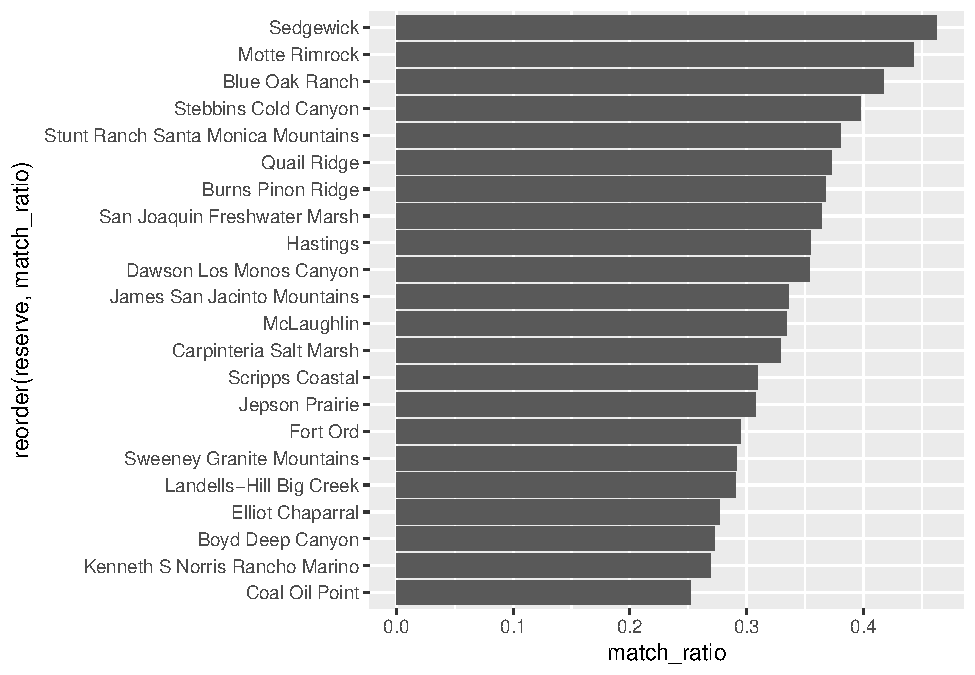
\includegraphics{conservancy_analysis_report_files/figure-latex/unnamed-chunk-7-1.pdf}

\begin{Shaded}
\begin{Highlighting}[]
\NormalTok{animalsComparisonTable }\OperatorTok\StringTok{ }
\StringTok{  }\KeywordTok{filter}\NormalTok{(match_ratio }\OperatorTok{>}\StringTok{ }\FloatTok{0.25}\NormalTok{) }\OperatorTok\StringTok{ }
\StringTok{  }\KeywordTok{ggplot}\NormalTok{(}\KeywordTok{aes}\NormalTok{(}\DataTypeTok{x =} \KeywordTok{reorder}\NormalTok{(reserve, match_ratio), }\DataTypeTok{y =}\NormalTok{ match_ratio)) }\OperatorTok{+}\StringTok{ }
\StringTok{  }\KeywordTok{geom_bar}\NormalTok{(}\DataTypeTok{stat =} \StringTok{"identity"}\NormalTok{) }\OperatorTok{+}
\StringTok{  }\KeywordTok{coord_flip}\NormalTok{()}
\end{Highlighting}
\end{Shaded}

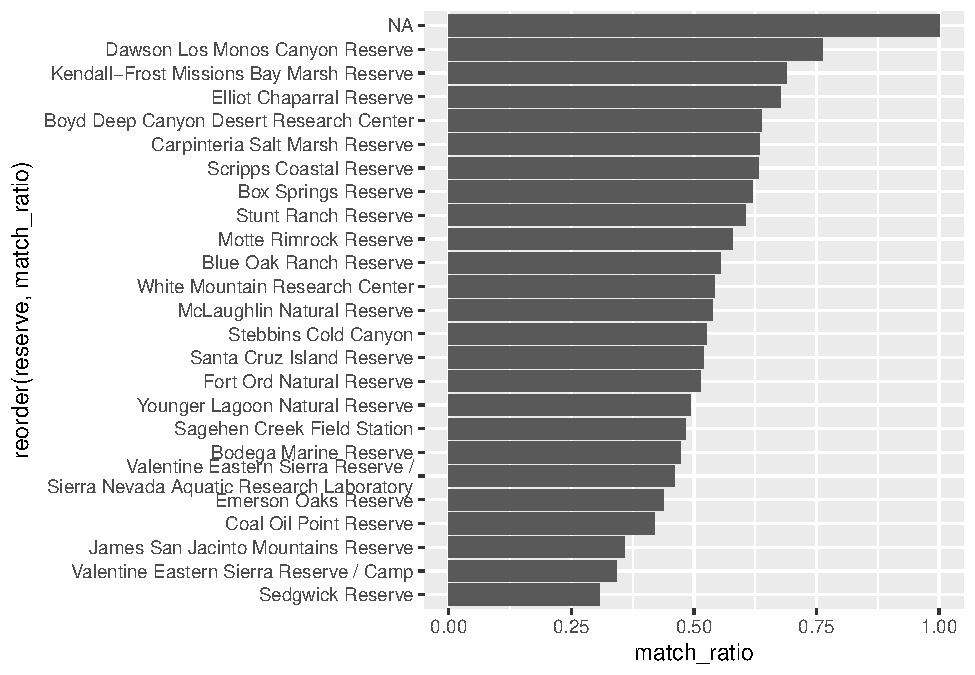
\includegraphics{conservancy_analysis_report_files/figure-latex/unnamed-chunk-7-2.pdf}

\subsection{Unique Plants and Animals}\label{unique-plants-and-animals}

\begin{Shaded}
\begin{Highlighting}[]
\NormalTok{uniquePlants <-}\StringTok{ }\NormalTok{conservancyPlantData }\OperatorTok\StringTok{ }\KeywordTok{anti_join}\NormalTok{(ucnrsPlantDataSubset, }\DataTypeTok{by =} \KeywordTok{c}\NormalTok{(}\StringTok{"genus"}\NormalTok{, }\StringTok{"species"}\NormalTok{, }\StringTok{"sublabel"}\NormalTok{))}
\NormalTok{uniqueAnimals <-}\StringTok{ }\NormalTok{conservancyAnimalData }\OperatorTok\StringTok{ }\KeywordTok{anti_join}\NormalTok{(ucnrsAnimalDataSubset, }\DataTypeTok{by =} \KeywordTok{c}\NormalTok{(}\StringTok{"genus"}\NormalTok{, }\StringTok{"species"}\NormalTok{, }\StringTok{"sublabel1"}\NormalTok{))}


\NormalTok{totalPlantsNum <-}\StringTok{ }\KeywordTok{nrow}\NormalTok{(conservancyPlantData)}
\NormalTok{uniquePlantsNum <-}\StringTok{ }\KeywordTok{nrow}\NormalTok{(uniquePlants)}

\NormalTok{totalAnimalsNum <-}\StringTok{ }\KeywordTok{nrow}\NormalTok{(conservancyAnimalData)}
\NormalTok{uniqueAnimalsNum <-}\StringTok{ }\KeywordTok{nrow}\NormalTok{(uniqueAnimals)}

\NormalTok{ratioUniquePlants <-}\StringTok{ }\NormalTok{uniquePlantsNum }\OperatorTok{/}\StringTok{ }\NormalTok{totalPlantsNum}
\NormalTok{ratioUniqueAnimals <-}\StringTok{ }\NormalTok{uniqueAnimalsNum }\OperatorTok{/}\StringTok{ }\NormalTok{totalAnimalsNum}

\NormalTok{rarePlants <-}\StringTok{ }\NormalTok{matchingPlantsReservesCombined }\OperatorTok\StringTok{ }\KeywordTok{filter}\NormalTok{(count }\OperatorTok{<}\StringTok{ }\DecValTok{4}\NormalTok{)}
\NormalTok{rarePlantsNum <-}\StringTok{ }\KeywordTok{nrow}\NormalTok{(rarePlants)}
\NormalTok{rareOrUniquePlantsNum <-}\StringTok{ }\NormalTok{uniquePlantsNum }\OperatorTok{+}\StringTok{ }\NormalTok{rarePlantsNum}

\NormalTok{rareAnimals <-}\StringTok{ }\NormalTok{matchingAnimalsReservesCombined }\OperatorTok\StringTok{ }\KeywordTok{filter}\NormalTok{(count }\OperatorTok{<}\StringTok{ }\DecValTok{4}\NormalTok{)}
\NormalTok{rareAnimalsNum <-}\StringTok{ }\KeywordTok{nrow}\NormalTok{(rareAnimals)}
\NormalTok{rareOrUniquePlantsNum <-}\StringTok{ }\NormalTok{uniqueAnimalsNum }\OperatorTok{+}\StringTok{ }\NormalTok{rareAnimalsNum}

\NormalTok{ratioRareOrUniquePlants <-}\StringTok{ }\NormalTok{rareOrUniquePlantsNum }\OperatorTok{/}\StringTok{ }\NormalTok{totalPlantsNum}
\NormalTok{ratioRareOrUniqueAnimals <-}\StringTok{ }\NormalTok{rareOrUniquePlantsNum }\OperatorTok{/}\StringTok{ }\NormalTok{totalAnimalsNum}


\NormalTok{ratioUniquePlants}
\end{Highlighting}
\end{Shaded}

\begin{verbatim}
## [1] 0.3744813
\end{verbatim}

\begin{Shaded}
\begin{Highlighting}[]
\NormalTok{ratioRareOrUniquePlants}
\end{Highlighting}
\end{Shaded}

\begin{verbatim}
## [1] 0.08921162
\end{verbatim}

\begin{Shaded}
\begin{Highlighting}[]
\NormalTok{ratioUniqueAnimals}
\end{Highlighting}
\end{Shaded}

\begin{verbatim}
## [1] 0.09631728
\end{verbatim}

\begin{Shaded}
\begin{Highlighting}[]
\NormalTok{ratioRareOrUniqueAnimals}
\end{Highlighting}
\end{Shaded}

\begin{verbatim}
## [1] 0.2436261
\end{verbatim}

\begin{Shaded}
\begin{Highlighting}[]
\NormalTok{uniquePlants}
\end{Highlighting}
\end{Shaded}

\begin{verbatim}
## # A tibble: 361 x 4
##    genus       species       separator_label sublabel   
##    <chr>       <chr>         <chr>           <chr>      
##  1 Allium      howellii      var.            howellii   
##  2 Allium      lacunosum     var.            davisiae   
##  3 Allium      peninsulare   var.            peninsulare
##  4 Rhus        aromatica     <NA>            <NA>       
##  5 Cicuta      douglasii     <NA>            <NA>       
##  6 Perideridia pringlei      <NA>            <NA>       
##  7 Chaenactis  glabriuscula  var.            megacephala
##  8 Chaenactis  santolinoides <NA>            <NA>       
##  9 Chaenactis  xantiana      <NA>            <NA>       
## 10 Crepis      acuminata     <NA>            <NA>       
## # ... with 351 more rows
\end{verbatim}

\begin{Shaded}
\begin{Highlighting}[]
\NormalTok{uniqueAnimals}
\end{Highlighting}
\end{Shaded}

\begin{verbatim}
## # A tibble: 34 x 4
##    genus         species      sublabel1    sublabel2
##    <chr>         <chr>        <chr>        <chr>    
##  1 Colinus       virginianus  <NA>         <NA>     
##  2 Falco         peregrinus   anatum       <NA>     
##  3 Porzana       Carolina     <NA>         <NA>     
##  4 Recurvirostra american     <NA>         <NA>     
##  5 Hydroprogne   caspia       <NA>         <NA>     
##  6 Strix         occidentalis occidentalis <NA>     
##  7 Aeronautes    vauxi        <NA>         <NA>     
##  8 Hylocichla    mustelina    <NA>         <NA>     
##  9 Myadestes     townsendii   <NA>         <NA>     
## 10 Setophaga     coronata     coronata     group    
## # ... with 24 more rows
\end{verbatim}

\begin{Shaded}
\begin{Highlighting}[]
\NormalTok{rarePlants}
\end{Highlighting}
\end{Shaded}

\begin{verbatim}
## # A tibble: 304 x 5
##    genus           species         sublabel   reserve_list           count
##    <chr>           <chr>           <chr>      <chr>                  <int>
##  1 Abies           concolor        <NA>       James San Jacinto Mou~     2
##  2 Acamptopappus   sphaerocephalus hirtellus  Sweeney Granite Mount~     1
##  3 Ailanthus       altissima       <NA>       McLaughlin, Quail Rid~     3
##  4 Allium          burlewii        <NA>       Boyd Deep Canyon, Jam~     2
##  5 Allium          fimbriatum      fimbriatum Boyd Deep Canyon, Bur~     3
##  6 Ambrosia        acanthicarpa    <NA>       Boyd Deep Canyon, Bur~     3
##  7 Amsinckia       intermedia      <NA>       Landells-Hill Big Cre~     1
##  8 Amsinckia       tessellata      tessellata Boyd Deep Canyon, Swe~     2
##  9 Ancistrocarphus filagineus      <NA>       McLaughlin, Motte Rim~     3
## 10 Anisocoma       acaulis         <NA>       Boyd Deep Canyon, Bur~     3
## # ... with 294 more rows
\end{verbatim}

\begin{Shaded}
\begin{Highlighting}[]
\NormalTok{rareAnimals}
\end{Highlighting}
\end{Shaded}

\begin{verbatim}
## # A tibble: 52 x 5
##    genus            species      sublabel1 reserve_list              count
##    <chr>            <chr>        <chr>     <chr>                     <int>
##  1 Actinemys        marmorata    <NA>      Angelo Coast Range Reser~     3
##  2 Alectoris        chukar       <NA>      Motte Rimrock Reserve, S~     2
##  3 Ammospermophilus leucurus     <NA>      Boyd Deep Canyon Desert ~     1
##  4 Amphispiza       bilineata    <NA>      Boyd Deep Canyon Desert ~     3
##  5 Anas             penelope     <NA>      Bodega Marine Reserve, C~     3
##  6 Aythya           marila       <NA>      Bodega Marine Reserve         1
##  7 Batrachoseps     nigriventris <NA>      Elliot Chaparral Reserve~     2
##  8 Botaurus         lentiginosus <NA>      Boyd Deep Canyon Desert ~     3
##  9 Bubulcus         ibis         <NA>      Boyd Deep Canyon Desert ~     3
## 10 Callisaurus      draconoides  <NA>      Boyd Deep Canyon Desert ~     2
## # ... with 42 more rows
\end{verbatim}


\end{document}
